\section{Physics}
One of the main requirements of the motor-generator set was its reciprocity. The model was to be robust and able to function as both a motor and generator with the same parts when operated backwards. Therefore, only a few laws unifying magnetic fluxes with electric fields are required to explain the functionality of the motor-generator kit.

    \subsection{Maxwell's Equations}
    Maxwell's Equations together form the foundation of classical electromagnetics.\\

        \begin{figure}[ht]
            \begin{center}
                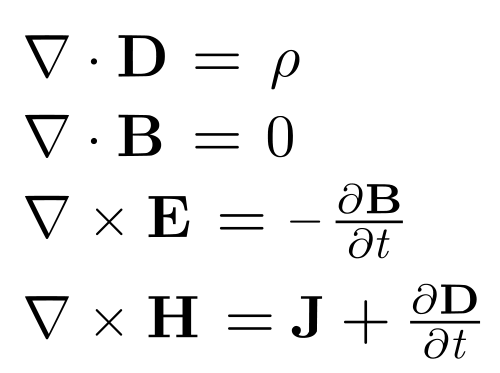
\includegraphics[width=0.6\textwidth]{figures/maxwell.png}
                \caption{Maxwell's Equations} \label{fig:maxwell}
            \end{center}
        \end{figure}

    \noindent
    Only one of these laws are required to explain the reciprocal functionality of the motor-generator kit - the third law - Faraday's Law of Induction.

    \subsection{Faraday's Law of Induction}
    Electromagnetic induction is the bidirectional process where a changing magnetic field around a conductor, or a conductor moving through a stationary magnetic field, generates (or induces) current.

        \begin{figure}[ht]
            \begin{center}
                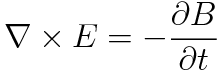
\includegraphics[width=0.3\textwidth]{figures/law_3.png}
                \caption{Faraday's Law of Induction} \label{fig:induction_law}
            \end{center}
        \end{figure}

    \subsection{Relating to Coils}
    Faraday's law of induction can be related to coils to demonstrate the relationship between the electromotive force (induced voltage) and the induced magnetic flux with Figure \ref{fig:coil_law}.\\

        \begin{figure}[ht]
            \begin{center}
                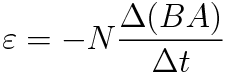
\includegraphics[width=0.3\textwidth]{figures/law_3c.png}
                \caption{Faraday's Law of Induction Relating to Coils} \label{fig:coil_law}
            \end{center}
        \end{figure}

    \noindent
    According to the law, a conductive coil rotating in a uniform magnetic field would induce current. Inversely, if current is supplied to the coil, a magnetic field is generated from it, demonstrated on Figure \ref{fig:coil}. Once the induced magnetic field properly aligns with the field lines of the already existing magnetic fields, the coil would begin repelling on same poles and attracting on the opposites, causing consistent rotations. The alignment of the fields that the models constructed were based on Figure \ref{fig:moving_coil}.

        \begin{figure}[ht]
            \begin{center}
                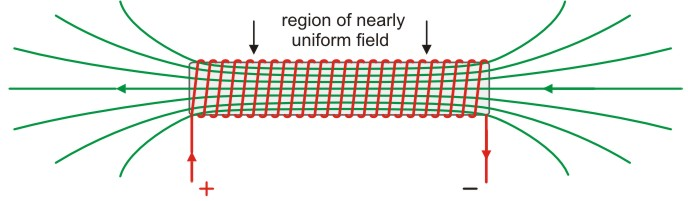
\includegraphics[width=0.43\textwidth]{figures/coil.jpg}
                \caption{Magnetic Field Lines Induced from Current flowing through Conductive Coil} \label{fig:coil}
            \end{center}
        \end{figure}

        \begin{figure}[ht]
            \centering

            \begin{subfigure}[b]{0.5\linewidth}
                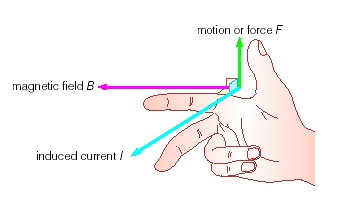
\includegraphics[width=0.8\textwidth]{figures/right_hand.jpg}
                \caption{Orthogonal Relationships Between \\Magnetic and Electric Fields}
            \end{subfigure}\hfill
            \begin{subfigure}[b]{0.5\linewidth}
                \centering
                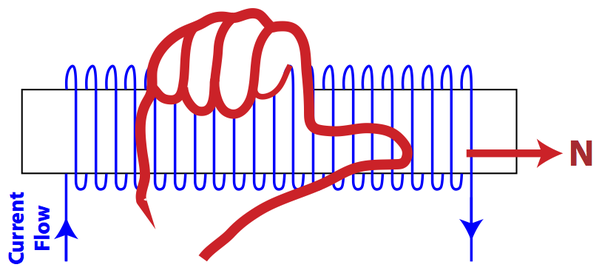
\includegraphics[width=0.8\textwidth]{figures/right_hand_coil.png} % first figure itself
                \caption{The Right-hand Rule Relating to the Direction \\of the Induced Magnetic Field}
            \end{subfigure}

            \begin{subfigure}[b]{0.5\linewidth}
                \centering
                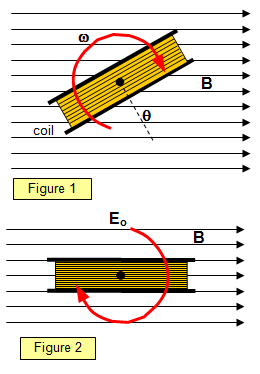
\includegraphics[width=0.8\textwidth]{figures/moving_coil.png} % second figure itself
                \caption{Motion of the Coils Used in the Final Models}
            \end{subfigure}
            \caption{Magnetic Field Lines driving the Motor-Generator Kit}
        \end{figure} \label{fig:moving_coil}

    \clearpage